\section{The hydration of formaldehyde in water}
\label{sec:bigexample}

In this section we describe in detail the hydration of formaldehyde in 
water~\footnote{Detailed description of the reaction is given in \cite{claydon}. 
The main path is on page 143, the base-catalysed  reaction is on page 713, and 
the acid-catalysed reaction in on page 343 of \cite{claydon}.} Formaldehyde 
is a good preservative and is well known for its use in preserving specimen samples. 
It also serves as an important building block in industrial processes and is therefore 
produced in large quantities. At room temperature, formaldehyde forms a colourless and smelly gas. 
Formaldehyde reacts with water molecules to form methanediol. The reaction is shown in 
Figure~\ref{fig:formal1}. It is reversible but it is much faster towards the methanediol, so 
the equilibrium contains mostly methanediol. It should be noted that other reactions are 
taking place in a solution of formaldehyde in water, however we consider only the interaction 
of formaldehyde with water molecules. The carbon atom of formaldehyde is not shown in 
Figure~\ref{fig:formal1} in line with a common convention. It resides at the point where 
the lines from the oxygen and the hydrogens
meet; we follow this convention in all other reaction diagrams. 
We use single lines to represent single bonds in all our reactions, and we use
double lines for double bonds, where two electron pairs are shared between atoms.

\begin{figure}[h!]
  \centering
    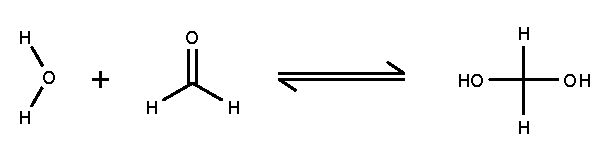
\includegraphics[width=0.6\textwidth]{formaldehyde1}
  \caption{Hydration of formaldehyde in water into methanediol}
  \label{fig:formal1}
\end{figure}

\subsection{The most common mechanism of the reaction}

A closer look at the reaction in Figure~\ref{fig:formal1} shows that the most common sequence 
of intermediate reactions leading to methanediol is the one given in Figure~\ref{fig:formal2}.
We now describe carefully its steps. The oxygen atom in one of the water molecules attacks the central 
carbon in the formaldehyde to form the intermediate 2 in Figure~\ref{fig:formal2}. Then one 
of the hydrogens of the positively charged oxygen is taken away by another water molecule 
in a proton transfer. This gives the intermediate 3. Finally, a proton is donated to the other 
oxygen in the intermediate 3 to give the final configuration 4.

\begin{figure}[h!]
  \centering
    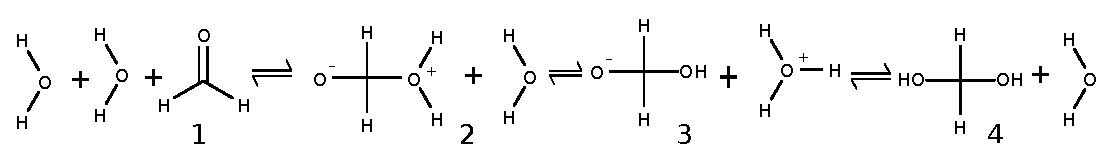
\includegraphics[width=1\textwidth]{formaldehyde2}
  \caption{The most common path through the hydration of formaldehyde}
  \label{fig:formal2}
\end{figure}

In order to model this reaction we need to understand what it is that makes it happen. 
The main factor is that the oxygen in the water is nucleophilic: it
tends to connect to another atomic nucleus. In the formaldehyde the oxygen attracts 
electrons towards itself, 
so the carbon has a positive charge. Now the oxygen in the water is attracted by this carbon 
and, due to its nucleophilicity, it forms a bond to the carbon. This bond is formed out of the electrons of one of the electrons in the oxygen so far not involved in bonding, so-called lone electron pairs. 
Since the carbon cannot have more than four bonds this reaction is compensated by 
the double bond in the formaldehyde becoming a single bond and the electrons from the double bond 
forming a lone pair on the oxygen, which now has three lone pairs. These movements are 
\emph{concerted}, namely they happen together without a stable intermediate state
and cannot be separated. So we have a continuous change between two tetracoordinate species through a pentacoordinate intermediate.  We have now reached the intermediate 2 in Figure~\ref{fig:formal2}. 

Looking at the intermediate 2, we can see that this has one oxygen which is negatively charged, 
because it has three lone pairs and a surplus of one electron. The other oxygen is positively 
charged, since it has three bonds and only one lone pair, therefore is missing an electron. 
The intermediate 2 reacts then with a water molecule. The water molecule is nucleophilic 
and has lone pairs for a bonding. It therefore can abstract one of the hydrogens on 
the positively charged oxygen. This leads to the intermediate 3 and a $\mathrm{H_3O}$ molecule, 
a water with an additional hydrogen and a positively charged oxygen.

Finally, a hydrogen can be re-donated to the negatively charged oxygen. Note that the re-donated 
hydrogen may not be the one which was originally attached to the oxygen. This transfer 
is possible since the oxygen in the $\mathrm{H_30}$ is electron-deficient and the negative oxygen 
is rich in electrons. We then get the substrate 4 which contains the final product 
methanediol, and water.

\subsection{Other paths through the reaction}
\label{sec:otherpaths}

There are other paths through the reaction of formaldehyde and water.
We assume that we now have a mixture of three water molecules and one formaldehyde molecule. 
This shall allow us to explore all other water-formaldehyde interactions. Two water molecules can interact 
to form $\mathrm{H_3O}$ and $\mathrm{HO}$. This is known as \emph{autoprotolysis of water} and is
described in detail in \cite{merevcomp2015}. These two molecules can be considered an acid and a base
respectively\footnote{There are slightly different definitions of acids and bases in the literature,
we use the general Bronsted-Lowry acid-base theory, which defines a base as a proton acceptor and 
an acid as a proton donor.}. Both bases and acids can interact with formaldehyde 
and thus produce methanediol by different mechanisms than those in the previous section.

\begin{figure}[h!]
  \centering
    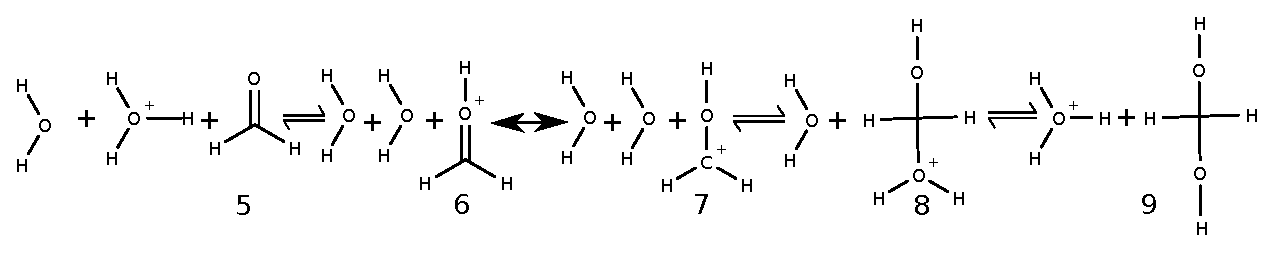
\includegraphics[width=1.0\textwidth]{formaldehyde_acid}
  \caption{Acid-catalysed hydration of formaldehyde in water.}
  \label{fig:acidcat}
\end{figure}

The acid-catalysed reaction is described in Figure~\ref{fig:acidcat}. Here the $\mathrm{H_3O}$ molecule,
which was formed during the autoprotolysis serves as the acid as it easily donates a proton. 
This proton can be donated to the oxygen in the formaldehyde, since this is slightly negatively charged, 
as we have seen. We then get the intermediate 6 in Figure~\ref{fig:acidcat}. The charge on the oxygen 
can ``move'' to the carbon by the electrons forming the bonds a lone pair on the oxygen. 
The real charge distribution is somewhere in between. We shall assume that the intermediates 6 and 7 
are somewhat  different structures, and we shall model the transition from 6 to 8 as a pair of 
concerted actions. Once the intermediate 8 is reached one of the protons from the oxygen in the
intermediate 8 can be abstracted by one of the water molecules, giving $\mathrm{H_3O}$ and
making it a catalytic process.

\begin{figure}[h!]
  \centering
    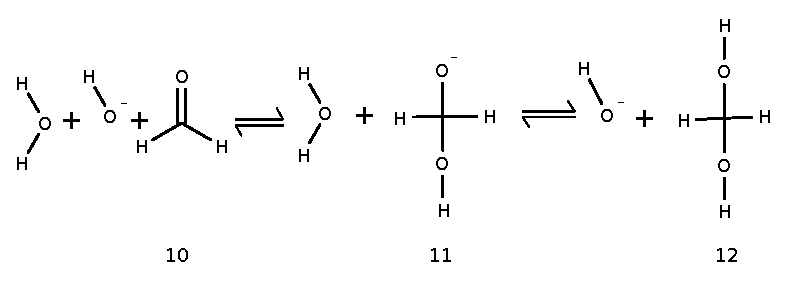
\includegraphics[width=0.7\textwidth]{formaldehyde_base}
  \caption{Base-catalysed hydration of formaldehyde in water.}
  \label{fig:basecat}
\end{figure}

The base-catalysed reaction in Figure~\ref{fig:basecat} starts with a water and a $\mathrm{HO^-}$ molecule, 
the base, which tends to accept protons very strongly. It can therefore interact with the carbon 
in the formaldehyde, which is similar to the water attacking the carbon. 
One of the bonds of the carbon-oxygen double bond is broken and the oxygen becomes negatively charged. 
This gives the intermediate 11 which is in fact the same as the intermediate 3 in 
Figure~\ref{fig:formal2}.
Then one of the protons of the water can be abstracted, and we obtain the methanediol and an 
$\mathrm{HO^⁻}$ molecule. Although this is the same structure as the original acid, it is made up 
from different atoms.  The process is considered catalytic since the $\mathrm{HO^⁻}$  molecule 
is retrieved at the end of the process.
\begin{figure}[h!]
\centering
      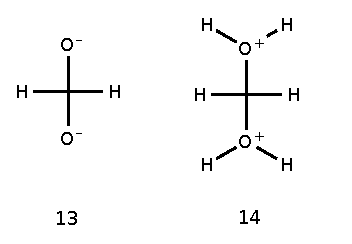
\includegraphics[width=.35\textwidth]{formaldehyde72}
        \caption{Other compounds possible in the reaction of formaldehyde with water.}
  \label{fig:misc}
\end{figure}

There are other ways that several molecules of water can react with formaldehyde to produce methanediol
and other byproducts. For example the base, $\mathrm{HO⁻}$, could directly interact with intermediate 7 
to form methanediol and two water molecules. 
Also, the two compounds given in Figure~\ref{fig:misc} can be created as intermediate products 
in the reaction. 

All possible reactions of a system of one formaldehyde and three water molecules are shown in
Figure~\ref{fig:formalallreal}. Although the direction of reactions are denoted with arrows, all 
reactions are reversible; the arrows merely indicate the direction to the final product.
We write FA for formaldehyde, W for water and MD for methanediol. Many of the intermediate compounds
are denoted by iX where $\mathrm{X}\in\{2,3,6,7,8,13,14\}$. 
Figure~\ref{fig:formalallreal} includes all intermediates from Figure~\ref{fig:acidcat} and 
Figure~\ref{fig:basecat}. The compounds in Figure~\ref{fig:misc} have only one path leading to them, 
and we could only move away from them by 
reverting these actions. This is because these compounds are the ``extreme'' states where there is 
either no hydrogen on an oxygen or both oxygens are fully saturated with two hydrogens. 
The resonance  between the intermediates i6 and i7 in Figure~\ref{fig:acidcat}  is represented 
by a dashed arrow.

\begin{figure}[t]
\psfrag{fawww}{${\mathrm{FA \paral W \paral W \paral W}}$}
\psfrag{fawhoh3o}{${\mathrm{FA \paral W \paral HO \paral H_3O}}$}
\psfrag{i6whow}{${\mathrm{i6 \paral W \paral HO \paral W}}$}
\psfrag{i8how}{${\mathrm{i8 \paral HO \paral W}}$}
\psfrag{mdhoh3o}{${\mathrm{MD \paral HO \paral H_3O}}$}
\psfrag{i2ww}{${\mathrm{i2 \paral W \paral W}}$}
\psfrag{i3h3ow}{${\mathrm{i3 \paral H_3O \paral W}}$}
\psfrag{mdww}{${\mathrm{MD \paral W \paral W}}$}
\psfrag{i6hohoh3o}{${\mathrm{i6 \paral HO \paral HO \paral H_3O}}$}
\psfrag{i7hohoh3o}{${\mathrm{i7 \paral HO \paral HO \paral H_3O}}$}
\psfrag{i7whow}{${\mathrm{i7 \paral W \paral HO \paral W}}$}
\psfrag{i14hoho}{${\mathrm{i14 \paral HO \paral HO}}$}
\psfrag{i13h3oh3o}{${\mathrm{i13 \paral H_3O \paral H_3O}}$}
\psfrag{i2hoh3o}{${\mathrm{i2 \paral H_3O \paral H_3O}}$}
  \centering
    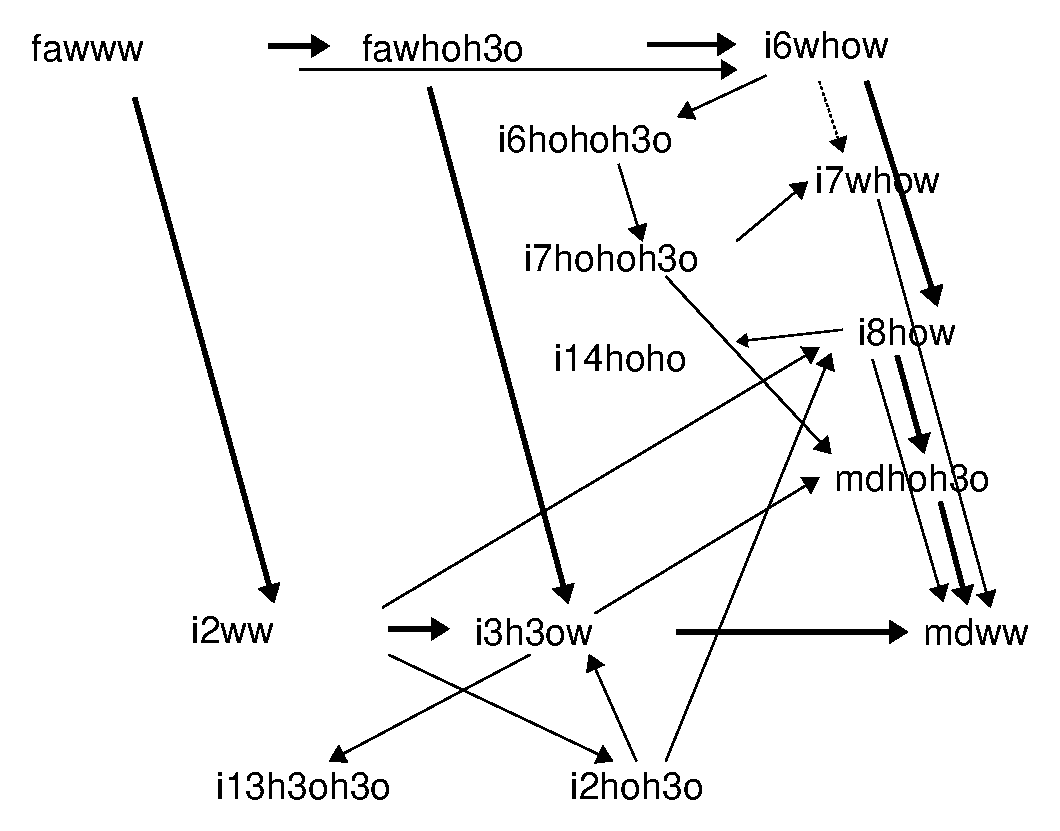
\includegraphics[width=1.0\textwidth]{formal_all_real2}
\caption{All possible reactions in a system of formaldehyde and three water molecules. 
The reactions displayed in more detail in Figure~\ref{fig:formal_graph} are denoted here by bold
arrows.}
  \label{fig:formalallreal}
\end{figure}

\Comment{
If, as it is normally done, the three possibilities are given separately, only the necessary molecules are taken into consideration. This is what we have done in Figure~\ref{fig:acidcat} and Figure~\ref{fig:basecat}, where only the base respectively acid and one water is shown. In our overall system we always have one water, one base and one acid. This means we get some additional paths. For example the base, $\mathrm{HO⁻}$, could directly interact with intermediate 7 to form methanediol and 2 water molecules. Figure~\ref{fig:formalallreal} shows all possible reactions in a system of formaldehyde and three water molecules. Actions are marked with an arrow to go from formaldehyde to methanediol, but all reactions are reversible. Figure~\ref{fig:formalallreal} includes all intermediates from Figure~\ref{fig:acidcat} and Figure~\ref{fig:basecat}. In addition two compounds given in Figure~\ref{fig:misc} can be created. These compounds have only one path leading to them, and we could only move away from them by reverting these actions. This is because these compounds are the ``extreme'' states where there is either no hydrogen on an oxygen or both oxygens are fully saturated with two hydrogens. In compounds where the two oxygens have different numbers of hydrogens we get different actions depending on which oxygen is involved. 
}

\Comment{
Figure~\ref{fig:formalallreal} is compiled from a chemical point of view - the nodes represent identical compounds. If these are identical processes in our calculus as well is not guaranteed. We will explore this difference in Section~\ref{sec:ccbwithsubscripts} further.

Notice there are other paths our calculus would enable. One example is an interaction of the methanediol, the final product, with a water molecule. Since the carbon has the action $p$ ready to perform and the oxygen in the water the action $n$ and $p,n$ is part of our synchronisation function there is nothing stopping this to happen. We have actually used a similar mechanism to get from 1 to 2 in Figure~\ref{fig:formal2}. A reason why this is not happening with methanediol is that the four groups around the carbon shield it from any interaction (as opposed to the three groups on the formaldehyde, of which two are relatively small hydrogens). So this is prevented by steric effect, effects due to atoms occupying space and preventing other atoms from moving.
}

\section{A CCB model of the hydration of formaldehyde in water}
\label{sec:formaldehydemodel}
We are now ready to model our reaction in CCB.
Figure~\ref{fig:formal_graph} shows in more detail the three main paths through our reaction 
that we described in the last section; these paths have been highlighted in bold in 
Figure~\ref{fig:formalallreal}. 

The initial state of the reaction is modelled by the composition of one 
formaldehyde FA three waters, written as $\mathrm{FA \paral W \paral W \paral W}$. 
The final products are methanediol $\mathrm{MD}$ and two waters,
written as $\mathrm{MD \paral W \paral W}$. The path via the intermediate molecules 2 and 3 
in Figure~\ref{fig:formal2} is via the nodes denoted by i2 and i3 in Figure~\ref{fig:formal_graph}.
The $\mathrm{FA \paral W \paral HO \paral H_3O}$ 
node is the result of an autoprotolysis. The base-catalysed and acid-catalysed reactions 
are put into the same diagram, again the intermediates i6 and i8 correspond to molecules 
in Figure~\ref{fig:acidcat}. 
%
%The subscripts in the transitions refer to the modelling done in the next paragraph. 
%
As we can see in Figure~\ref{fig:formal_graph} the reactions are driven completely by 
concerted actions. 
%
%TODO: We note that the transition from the intermediate 6 to 8 is somewhat
%different to other transitions, and may need to be represented more specifically in the future. 
%The remaining transitions are handled as concerted actions by our calculus.

\begin{figure}[t]
\psfrag{l1}{${\scriptstyle\{np[11],\underline{c_4o_2}[4]\}}$}
\psfrag{l2}{${\scriptstyle\{np[12],\underline{h_3o_3}[5]\}}$}
\psfrag{l3}{${\scriptstyle\{np[13],\underline{h_5o_5}[12]\}}$}
\psfrag{l4}{${\scriptstyle\{np[12],\underline{h_3o_3}[5]\}}$}
\psfrag{l5}{${\scriptstyle\{np[11],\underline{c_4o_2}[4]\}}$}
\psfrag{l6}{${\scriptstyle\{np[13],\underline{h_5o_5}[7]\}}$}
\psfrag{l7}{${\scriptstyle\{np[11],\underline{c_4o_2}[4]\}}$}
\psfrag{l8}{${\scriptstyle\{np[14],\underline{h_6o_6}[8]\}}$}
\psfrag{l9}{${\scriptstyle\{np[5],\underline{h_8o_8}[14]\}}$}

\psfrag{fawww}{${\mathrm{FA \paral W \paral W \paral W}}$}
\psfrag{fawhoh3o}{${\mathrm{FA \paral W \paral HO \paral H_3O}}$}
\psfrag{i6whow}{${\mathrm{i6 \paral W \paral HO \paral W}}$}
\psfrag{i8how}{${\mathrm{i8 \paral HO \paral W}}$}
\psfrag{mdhoh3o}{${\mathrm{MD \paral HO \paral H_3O}}$}
\psfrag{i2ww}{${\mathrm{i2 \paral W \paral W}}$}
\psfrag{i3h3ow}{${\mathrm{i3 \paral H_3O \paral W}}$}
\psfrag{mdww}{${\mathrm{MD \paral W \paral W}}$}

\centering
    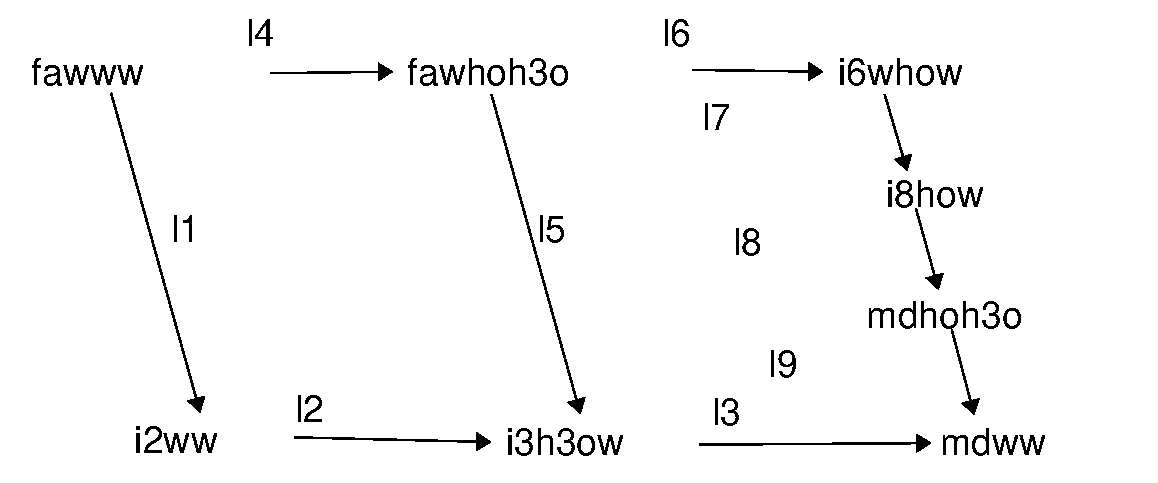
\includegraphics[width=1.0\textwidth]{formal_all}
\caption{The three main reaction paths in the hydration of formaldehyde.}
\label{fig:formal_graph}
\end{figure}

We model the formaldehyde molecule $\mathrm{CH_2O}$ and the three water molecules $\mathrm{H_2O}$
as appropriate compositions of their atoms, namely hydrogen, oxygen and carbon. We use our 
general prefixing operator to define these atoms: 
$$\begin{array}{lll}
H & \bydef & (h;p).H'\\
O & \bydef & (o,o,n).O'\\
C & \bydef & (c,c,c,c;p).C'
\end{array}$$
Carbon has four strong actions $c$, representing the potential for four covalent bonds, and 
a weak action $p$, standing for a positive partial charge. 
The oxygen can have up to three bonds. Normally is has two bonds, however, if a suitable reaction 
partner is close, an additional weak bond is available. We use therefore the simple prefixing operator
to model it, with one weak action $n$ standing for the potential for a negative partial charge. 
A partial charge means that a part or parts of a molecule have an electric charge, even though 
the molecule as a whole is neutrally charged. These uneven charge distributions enable 
many reactions by allowing another molecule to attack a partially charged part.
The hydrogen has one strong bond, and we use additionally a weak action $p$ to represent 
that it can become positively charged. Processes $H'$, $O'$, and $C'$ represent 
unspecified further behaviour of the respective atoms.

Since our reaction involves multiple copies of $H$ and $O$ we shall adopt a subscript notation 
to denote distinct copies of the same process. Both action labels and process names will be
subscripted. For example, $H_1\bydef (h_1;p).H_1'$ and $H_2\bydef (h_2;p).H_2'$ are two copies
of hydrogen $H$. 
We shall abstract away these subscripts in Section~\ref{chem-eq}, where we introduce
informally chemical equivalence.  
Also, the copies of actions $c$ of carbon will also be subscripted.
% to ``tell them apart". 

The synchronisation function $\gamma$ is defined on subscripted actions as follows:
%
$$\begin{array}{ l c l l }
\gamma(c_i,h_j) & = & c_ih_j \quad & i \in \{1,\ldots, 4\}, j\in\{1,\ldots,8\} \\
\gamma(h_i,o_j) & = & h_io_j \quad & i \in \{1,\ldots, 8\}, j\in\{1,\ldots,6\}  \\
\gamma(c_i,o_j) & = & c_io_j \quad & i \in \{1,\ldots, 4\}, j\in\{1,\ldots,6\} \\
\gamma(c_i,n) & = & c_in & i \in \{1,\ldots, 4\} \\
\gamma(h_i,n) & = & h_in & i \in \{1,\ldots,8\}  \\
\gamma(n,p) & = & np &  \\
\end{array}$$
Now we are ready to model $\mathrm{H_2O}$ and $\mathrm{CH_2O}$ molecules. A water molecule is modelled 
simply as a composition of two copies of the hydrogen process with one copy of oxygen; see below. 
%
\Comment{
\Stefan{The restrictions ensure that the molecules form as desired and once they exist only 
communications on weak actions $n$ and $P$ happen.  Of course the atoms could react to form another 
set of molecules, but we assume a particular set of initial reactions to get the starting molecules 
for our reaction.} 
}
The restriction of actions $h_i$ and $o_i$, for $i\in\{3,4\}$, ensures that actions such as 
$h_3[5]$ cannot be undone alone but only together with their partners $o_3[5]$. This happens via
undoing of $h_3o_3[5]$ bond. Correspondingly, when
any of these actions is fresh they can only happen together with their partners (as prescribed by
the communication function $\gamma$), and not alone. 
We also restrict $np$ to stop self-bonding of water's hydrogens with its oxygen.
%and that we do not allow $n$ and $p$ to bond, or refer to RC15 paper
%
$$\begin{array}{l}
((h_3[5];p).H'_3 \paral (h_4[6];p).H'_4 \paral (o_3[5],o_4[6],n).O'_2)
  \setminus\{h_3,h_4,o_3,o_4, np\} \\
\end{array}$$
The formaldehyde molecule is modelled by
$$\begin{array}{l}
(((c_1[1],c_2[2],c_3[3],c_4[4];p).C' \paral (h_1[1];p).H'_1 \paral (h_2[2];p).H'_2 \paral
(o_1[3],o_2[4],n).O'_1)\\
  \quad \setminus\{c_1,c_2,c_3,c_4,h_1,h_2,o_1,o_2,np,\underline{c_{1}h_{1}}, \underline{c_{2}h_{2}},
  \}
\end{array}$$
We restrict the appropriate versions of the $c_i, o_j$ and $h_k$ actions, for
all $i,j$ and $k$, meaning that we do not allow the creation of new bonds (involving these actions)
between different molecules as single acts of synchronisation. Such new bonds will be created
via concerted actions and (almost) always via the weak $np$ bonds which will then get promoted
to strong bonds.

We also restrict $\underline{c_i h_i}$ for $i\in\{1,2\}$. It prevents
breaking any of the bonds between $C_1$ and its hydrogens $H_1$ and $H_2$.
This serves two purposes. Firstly, it makes sure that once we have done the $p$ action of
the carbon, we will break one of the bonds between the carbon and the oxygen. This is justified
since in reality it is one of the oxygen bonds which is broken, so this models the reality closely.
Secondly, it also prevents $O_2$ or $O_3$ from abstracting $H_1$ or $H_2$ from the carbon.
Note that $\underline{h_i}$, $\underline{o_j}$ and $\underline{n}$ are not restricted in FA and 
in W: this allows us to break bonds involving these actions as a part of concerted
actions.

The four molecules of the reaction are now composed in parallel:
$$(\mathrm{CH_2O \paral H_2O \paral H_2O \paral H_2O})\setminus \{n,p\}$$
We restrict actions $n$ and $p$, so that they
cannot happen separately from each other but only together within this system of processes. 

The main path through the reaction require only two copies of water so we start 
with the following initial state, where keys $1, \ldots, 8$ specify the existing
initially bonds of formaldehyde and the two waters.
\begin{flalign*}
&(((c_1[1],c_2[2],c_3[3],c_4[4];p).C' \paral (h_1[1];p).H'_1 \paral (h_2[2];p).H'_2 \paral 
(o_1[3],o_2[4],n).O'_1) \\
 & \qquad  \setminus\{c_1,c_2,c_3,c_4,h_1,h_2,o_1,o_2,np,\underline{c_{1}h_{1}}, \underline{c_{2}h_{2}}\} \\
&\paral ((h_3[5];p).H'_3 \paral (h_4[6];p).H'_4 \paral (o_3[5],o_4[6],n).O'_2) 
  \setminus\{h_3,h_4,o_3,o_4,np\} \\
&\paral ((h_5[7];p).H'_5 \paral (h_6[8];p).H'_6 \paral (o_5[7],o_6[8],n).O'_3) 
  \setminus\{h_5,h_6,o_5,o_6,np\} ) \; \setminus \{n,p\}
\end{flalign*}
%
In order to simplify the display of transitions or rewrites of this process we omit the four
restrictions and write the initial process simply as
%
\begin{flalign*}
&(c_1[1],c_2[2],c_3[3],c_4[4];p).C' \paral (h_1[1];p).H'_1 \paral (h_2[2];p).H'_2 \paral (o_1[3],o_2[4],n).O'_1 
   \\
&\paral (h_3[5];p).H'_3 \paral (h_4[6];p).H'_4 \paral (o_3[5],o_4[6],n).O'_2 
   \\
&\paral (h_5[7];p).H'_5 \paral (h_6[8];p).H'_6 \paral (o_5[7],o_6[8],n).O'_3 
%\; \setminus L
\end{flalign*}
%where $L=\{c_1,c_2,c_3,c_4,h_1,h_2,h_3,h_4,h_5,h_6,o_1,o_2,o_3,o_4,o_5,o_6,n,p,
%\underline{c_{1}h_{1}}, \underline{c_{2}h_{2}}\}$.
remembering that the restrictions are still there.

\subsection{The main path through the reaction}
We first consider the reaction steps in Figure~\ref{fig:formal2}, following the path via 
$\mathrm{i3 \paral H_3O \paral W}$ and $\mathrm{i2 \paral W \paral W}$
in Figures~\ref{fig:formalallreal} and \ref{fig:formal_graph}. The first step is the $n,p$ 
reaction between $C_1$ and $O_2$ or $O_3$. 
Note that there are other $n,p$ reactions that are allowed by our model. 
%
% introducing a restriction of np stops this now:
\Comment{For example, the $n,p$ reaction between $O_1$ and $C$. 
If $O_1$ reacted with $C$, this would force the breaking of one of 
the bonds $1,\ldots,4$ of the carbon. Since restriction of $\underline{c_i h_i}$, for $i\in\{1,2\}$,
prevents dissolving of bonds 1 and 2, one of the bonds 3 or 4 will be broken. So, we will
end up with two bonds between $C$ and $O_1$ as before. Hence, this would not lead to an
effective change, so this case is omitted.
}
We could have $O_2$ getting a hydrogen from $O_3$,
or vice versa, which is the autoprotolysis of water which we have mentioned before. 
We shall discuss this 
further later on. Also $O_1$ could pull one of the hydrogens from one of the water molecules:
again we shall discuss it later. 

Returning to the first step of our reaction, we have 
$O_2$ bonding with $C$ with the key $11$. This is followed immediately by breaking of the bond 3 or 4 
by the rule \rulename{concert}.
% applied to a process of the form $(s;b).P$ in parallel with another process. 
Note that
breaking of 1 or 2 is not possible because of the restriction of $c_1h_1$ and $c_2h_2$. 
We break the bond 4 and get a transition by concerted actions: 
we create the bond $np[11]$ and break the bond $\underline{c_4o_2}[4]$. Henceforth
we shall write the name of the target of a transition below the transition,
using the names that appear in Figures~\ref{fig:formalallreal}-\ref{fig:formal_graph}.
Here, for example, the compound resulting from
this transition is $\mathrm{i2 \paral W }$ but since in general we have an extra water W,
we write $\mathrm{i2 \paral W \paral W}$.
\begin{flalign*}
&\xrightarrow{\{np[11],\underline{c_4o_2}[4]\}}
	(c_1[1],c_2[2],c_3[3],c_4;p[11]).C' \paral (h_1[1];p).H'_1 \paral (h_2[2];p).H'_2 \paral \\
&\qquad (o_1[3],o_2,n).O'_1 \paral (h_3[5];p).H'_3 \paral (h_4[6];p).H'_4 \paral (o_3[5],o_4[6],n[11]).O'_2 \\
&\paral (h_5[7];p).H'_5 \paral (h_6[8];p).H'_6 \paral (o_5[7],o_6[8],n).O'_3 % ) \setminus L \qquad 
\end{flalign*}
\hfill{$\mathrm{i2 \paral W \paral W}$}
\\
Now the \rulename{prom} rewrite rule must be applied before we derive the next concerted transition: we promote 
the weak bond 11 of the carbon to a stronger bond on $c_4$, which has become available:
%
\begin{flalign*}
&\Tran{} \; ((c_1[1],c_2[2],c_3[3],c_4[11];p).C' \paral (h_1[1];p).H'_1 \paral (h_2[2];p).H'_2  \\
&\paral (o_1[3],o_2,n).O'_1 \paral (h_3[5];p).H'_3 \paral (h_4[6];p).H'_4 \paral (o_3[5],o_4[6],n[11]).O'_2 \\
&\paral (h_5[7];p).H'_5 \paral (h_6[8];p).H'_6 \paral (o_5[7],o_6[8],n).O'_3 ) \setminus L \qquad
\end{flalign*}
\hfill{$\mathrm{i2 \paral W \paral W}$}
\\
%We note that $O_1$ is now negatively charged (it has only one bond), but we do not need to 
%consider it to get our desired result. 
The next step is to form a bond between $O_3$ and
either $H_3$ or $H_4$. We bond with $H_3$ with the key 12 and break the bond 5, producing a pair
of concerted actions. We then move a weak bond 11 on $n$ in $O_2$ to a stronger bond
on $o_3$ (which has become available) by rewrite rule move-r. We also promote the weak bond 12 in $H_3$ 
to a strong bond on $h_3$ by rewrite rule \rulename{prom}, giving overall this transition:
%
\begin{flalign*}
&\xrightarrow{\{np[12],\underline{h_3o_3}[5]\}}
	(c_1[1],c_2[2],c_3[3],c_4[11];p).C' \paral (h_1[1];p).H'_1 \paral (h_2[2];p).H'_2 \paral \\
&\qquad (o_1[3],o_2,n).O'_1 \paral (h_3[12];p).H'_3 \paral (h_4[6];p).H'_4 \paral (o_3[11],o_4[6],n).O'_2 \\
&\paral (h_5[7];p).H'_5 \paral (h_6[8];p).H'_6 \paral (o_5[7],o_6[8],n[12]).O'_3 %) \setminus L \qquad 
\end{flalign*}
\hfill{$\mathrm{i3 \paral H_3O \paral W}$}
\\

The next step is a proton transfer from $O_3$ to $O_1$. We transfer $H_5$ (but we could have used 
$H_6$ or $H_3$ since they all have the $p$ action ready). 
%That also $H_3$ can do so is thanks to our new calculus, since it has done some actions before, 
%but appears the same as the other hydrogens bonded to $O_3$. 
Performing the transfer of $H_5$ from $O_3$ to $O_1$ (and breaking the bond 12), we obtain the following:
%
\begin{flalign*}
&\xrightarrow{\{np[13],\underline{h_5o_5}[12]\}}
	(c_1[1],c_2[2],c_3[3],c_4[11];p).C' \paral (h_1[1];p).H'_1 \paral (h_2[2];p).H'_2 \paral \\
&\qquad (o_1[3],o_2,n[13]).O'_1 \paral (h_3;p[13]).H'_3 \paral (h_4[6];p).H'_4 \paral (o_3[11],o_4[6],n).O'_2 \\
&\paral (h_5[7];p).H'_5 \paral (h_6[8];p).H'_6 \paral (o_5[7],o_6[8],n).O'_3 %) \setminus L \qquad 
\end{flalign*}
\hfill{$\mathrm{MD \paral W \paral W}$}
\\
and promoting and moving the bond 13 in $H_3$ and $O_1$, respectively, to strong bonds 
we obtain the final product (methanediol $\mathrm{CH_2(OH)_2}$) and two waters:
%
\begin{flalign*}
	&\Tran{}\ (c_1[1],c_2[2],c_3[3],c_4[11];p).C' \paral (h_1[1];p).H'_1 \paral (h_2[2];p).H'_2\\
& \paral (o_1[3],o_2[13],n).O'_1 \paral (h_3[13];p).H'_3 \paral (h_4[6];p).H'_4 \paral (o_3[11],o_4[6],n).O'_2 \\
&\paral (h_5[7];p).H'_5 \paral (h_6[8];p).H'_6 \paral (o_5[7],o_6[8],n).O'_3 %) \setminus L \qquad
\end{flalign*}
\hfill{$\mathrm{MD \paral W \paral W}$}
%

\noindent
Note that the $n,p$ actions are ready again and all the existing bonds are on strong actions. 
So we now can reverse the reaction by $O_3$ abstracting a hydrogen from $H_4$ or $H_5$, and 
all the way to the initial state.
Moreover, let us inspect the bonds 4, 5 and 7 which are broken during the reaction. The bonds were formed during the initial bonding of the atoms. They are broken as a
result of application of our new general prefixing operator. This operator enables the reaction 
to work forwards without external control. Indeed the original order of the formation of 
the bonds is completely irrelevant for the reaction to work.

\subsection{The base-catalysed path}

We now consider the base-catalysed path described in Figure~\ref{fig:basecat}. The path is via  
$\mathrm{FA \paral W \paral HO \paral H_3O}$ and  $\mathrm{i3 \paral H_3O \paral W}$  to
$\mathrm{MD \paral W \paral W}$ in Figures~\ref{fig:formalallreal}-\ref{fig:formal_graph}. 
The path needs three water molecules. We shall show the application of the promotion or move 
rules without explaining them in detail. We start with the initial system (remembering that
restrictions are not shown):
\begin{flalign*} 
&(c_1[1],c_2[2],c_3[3],c_4[4];p).C' \paral (h_1[1];p).H'_1 \paral (h_2[2];p).H'_2 \paral 
	(o_1[3],o_2[4],n).O'_1 \\
&\paral (h_3[5];p).H'_3 \paral (h_4[6];p).H'_4 \paral (o_3[5],o_4[6],n).O'_2 
   \\
&\paral (h_5[7];p).H'_5 \paral (h_6[8];p).H'_6 \paral (o_5[7],o_6[8],n).O'_3 
   \\
&\paral (h_7[9];p).H'_7 \paral (h_8[10];p).H'_8 \paral (o_7[9],o_8[10],n).O'_4 
  %\; \setminus L \qquad 
\end{flalign*}
\hfill{$\mathrm{FA \paral W \paral W \paral W}$}
\\
%
\noindent
\begin{flalign*}
&\xrightarrow{\{np[12],\underline{h_3o_3}[5]\}}(c_1[1],c_2[2],c_3[3],c_4[4];p).C' \paral (h_1[1];p).H'_1 \paral (h_2[2];p).H'_2   \\
& \paral (o_1[3],o_2[4],n).O'_1 \paral (h_3;p[12]).H'_3 \paral (h_4[6];p).H'_4 \paral (o_3,o_4[6],n).O'_2 
   \\
&\paral (h_5[7];p).H'_5 \paral (h_6[8];p).H'_6 \paral (o_5[7],o_6[8],n[12]).O'_3 
   \\
&\paral (h_7[9];p).H'_7 \paral (h_8[10];p).H'_8 \paral (o_7[9],o_8[10],n).O'_4 
  %\; \setminus L \qquad
\end{flalign*}
%\hfill{$\mathrm{FA \paral W \paral HO \paral H_3O}$}
%\\
\begin{flalign*}
&\Tran{}(c_1[1],c_2[2],c_3[3],c_4[4];p).C' \paral (h_1[1];p).H'_1 \paral (h_2[2];p).H'_2
   \\
& \paral (o_1[3],o_2[4],n).O'_1 \paral (h_3[12];p).H'_3 \paral (h_4[6];p).H'_4 \paral (o_3,o_4[6],n).O'_2 
   \\
&\paral (h_5[7];p).H'_5 \paral (h_6[8];p).H'_6 \paral (o_5[7],o_6[8],n[12]).O'_3 
   \\
&\paral (h_7[9];p).H'_7 \paral (h_8[10];p).H'_8 \paral (o_7[9],o_8[10],n).O'_4 
  %\; \setminus L \qquad
\end{flalign*}
\hfill{$\mathrm{FA \paral W \paral HO \paral H_3O}$}
\\
\begin{flalign*}
&\xrightarrow{\{np[11],\underline{c_4o_4}[4]\}}(c_1[1],c_2[2],c_3[3],c_4;p[11]).C' \paral (h_1[1];p).H'_1 \paral (h_2[2];p).H'_2 
   \\
& \paral (o_1[3],o_2,n).O'_1 \paral (h_3[12];p).H'_3 \paral (h_4[6];p).H'_4 \paral (o_3,o_4[6],n[11]).O'_2 
   \\
&\paral (h_5[7];p).H'_5 \paral (h_6[8];p).H'_6 \paral (o_5[7],o_6[8],n[12]).O'_3 
   \\
&\paral (h_7[9];p).H'_7 \paral (h_8[10];p).H'_8 \paral (o_7[9],o_8[10],n).O'_4 
  %\; \setminus L \qquad
\end{flalign*}
%\hfill{$\mathrm{i3 \paral H_3O \paral W}$}
%\\
\begin{flalign*}
	&\Tran{}(c_1[1],c_2[2],c_3[3],c_4[11];p).C' \paral (h_1[1];p).H'_1 \paral (h_2[2];p).H'_2 
   \\
& \paral (o_1[3],o_2,n).O'_1 \paral (h_3[12];p).H'_3 \paral (h_4[6];p).H'_4 \paral (o_3[11],o_4[6],n).O'_2 
   \\
&\paral (h_5[7];p).H'_5 \paral (h_6[8];p).H'_6 \paral (o_5[7],o_6[8],n[12]).O'_3 
   \\
&\paral (h_7[9];p).H'_7 \paral (h_8[10];p).H'_8 \paral (o_7[9],o_8[10],n).O'_4 
  %\; \setminus L \qquad
\end{flalign*}
\hfill{$\mathrm{i3 \paral H_3O \paral W}$}
\\
\begin{flalign*}
&\xrightarrow{\{np[13],\underline{h_3n}[12]\}}(c_1[1],c_2[2],c_3[3],c_4[11];p).C' \paral (h_1[1];p).H'_1 \paral (h_2[2];p).H'_2 
   \\
&\paral (o_1[3],o_2,n[13]).O'_1 \paral (h_3;p[13]).H'_3 \paral (h_4[6];p).H'_4 \paral (o_3[11],o_4[6],n).O'_2 
   \\
&\paral (h_5[7];p).H'_5 \paral (h_6[8];p).H'_6 \paral (o_5[7],o_6[8],n).O'_3 
   \\
&\paral (h_7[9];p).H'_7 \paral (h_8[10];p).H'_8 \paral (o_7[9],o_8[10],n).O'_4 
  %\; \setminus L \qquad
\end{flalign*}
%\hfill{$\mathrm{MD \paral W \paral W}$}
%\\
\begin{flalign*}
&\Tran{}(c_1[1],c_2[2],c_3[3],c_4[11];p).C' \paral (h_1[1];p).H'_1 \paral (h_2[2];p).H'_2
   \\
& \paral (o_1[3],o_2[13],n).O'_1 \paral (h_3[13];p).H'_3 \paral (h_4[6];p).H'_4 \paral (o_3[11],o_4[6],n).O'_2 
   \\
&\paral (h_5[7];p).H'_5 \paral (h_6[8];p).H'_6 \paral (o_5[7],o_6[8],n).O'_3
   \\
&\paral (h_7[9];p).H'_7 \paral (h_8[10];p).H'_8 \paral (o_7[9],o_8[10],n).O'_4 
  %\; \setminus L \qquad
\end{flalign*}
\hfill{$\mathrm{MD \paral W \paral W}$}
\\
We have reached the final state of the reaction: a methanediol with two waters. Notice 
that the methanediol
process is identical (including keys) to the  methanediol process in the main path.
%
\subsection{The acid-catalysed path}

Next we consider the acid-catalysed path described in Figure~\ref{fig:acidcat}. The path is via
$\mathrm{i6 \paral W \paral HO \paral W}$ and $\mathrm{i8 \paral HO \paral W}$ in 
Figures~\ref{fig:formalallreal}--\ref{fig:formal_graph}.  The path uses three water molecules 
as in the base-catalysed path. We shall apply the promotion or move rules as needed.
We start with the initial system:
\begin{flalign*}
&(c_1[1],c_2[2],c_3[3],c_4[4];p).C' \paral (h_1[1];p).H'_1 \paral (h_2[2];p).H'_2  
   \\
&\paral (o_1[3],o_2[4],n).O'_1 \paral (h_3[12];p).H'_3 \paral (h_4[6];p).H'_4 \paral (o_3,o_4[6],n).O'_2 
   \\
&\paral (h_5[7];p).H'_5 \paral (h_6[8];p).H'_6 \paral (o_5[7],o_6[8],n[12]).O'_3 
\\
&\paral (h_7[9];p).H'_7 \paral (h_8[10];p).H'_8 \paral (o_7[9],o_8[10],n).O'_4 %  \; \setminus L \qquad 
\end{flalign*}
\hfill{$\mathrm{FA \paral W \paral HO \paral H_3O}$}
\\
\begin{flalign*}
&\xrightarrow{\{np[13],\underline{h_5o_5}[7]\}}(c_1[1],c_2[2],c_3[3],c_4[4];p).C' \paral (h_1[1];p).H'_1 \paral (h_2[2];p).H'_2
   \\
& \paral (o_1[3],o_2[4],n[13]).O'_1 \paral (h_3[12];p).H'_3 \paral (h_4[6];p).H'_4 \paral (o_3,o_4[6],n).O'_2 
   \\
&\paral (h_5;p[13]).H'_5 \paral (h_6[8];p).H'_6 \paral (o_5,o_6[8],n[12]).O'_3 
\\
&\paral (h_7[9];p).H'_7 \paral (h_8[10];p).H'_8 \paral (o_7[9],o_8[10],n).O'_4  % \; \setminus L \qquad
\end{flalign*}
%\hfill{$\mathrm{i6 \paral W \paral HO \paral W}$}
%\\
\begin{flalign*}
&\Tran{}(c_1[1],c_2[2],c_3[3],c_4[4];p).C' \paral (h_1[1];p).H'_1 \paral (h_2[2];p).H'_2
   \\
& \paral (o_1[3],o_2[4],n[13]).O'_1 \paral (h_3[12];p).H'_3 \paral (h_4[6];p).H'_4 \paral (o_3,o_4[6],n).O'_2 
   \\
&\paral (h_5[13];p).H'_5 \paral (h_6[8];p).H'_6 \paral (o_5[12],o_6[8],n).O'_3 
   \\
&\paral (h_7[9];p).H'_7 \paral (h_8[10];p).H'_8 \paral (o_7[9],o_8[10],n).O'_4 %\; \setminus L \qquad
\end{flalign*}
\hfill{$\mathrm{i6 \paral W \paral HO \paral W}$}
\\
The last rewrite is by rule \rulename{move-r}. The reaction continues as follows:

\begin{flalign*}
&\xrightarrow{\{np[11], \underline{c_4o_2}[4]\}}(c_1[1],c_2[2],c_3[3],c_4;p[11]).C' \paral (h_1[1];p).H'_1 \paral (h_2[2];p).H'_2
   \\
   & \paral (o_1[3],o_2,n[13]).O'_1 \paral (h_3[12];p).H'_3 \paral (h_4[6];p).H'_4 \paral (o_3,o_4[6],n).O'_2 
   \\
&\paral (h_5[13];p).H'_5 \paral (h_6[8];p).H'_6 \paral (o_5[12],o_6[8],n[11]).O'_3 
\\
&\paral (h_7[9];p).H'_7 \paral (h_8[10];p).H'_8 \paral (o_7[9],o_8[10],n).O'_4   %\; \setminus L \qquad
\end{flalign*}
%\hfill{$\mathrm{i8 \paral HO \paral W}$}
%\\
\begin{flalign*}
&\Tran{}(c_1[1],c_2[2],c_3[3],c_4[11];p).C' \paral (h_1[1];p).H'_1 \paral (h_2[2];p).H'_2 
   \\
&\paral (o_1[3],o_2[13],n).O'_1 \paral (h_3[12];p).H'_3 \paral (h_4[6];p).H'_4 \paral (o_3,o_4[6],n).O'_2 
   \\
&\paral (h_5[13];p).H'_5 \paral (h_6[8];p).H'_6 \paral (o_5[12],o_6[8],n[11]).O'_3 
\\
&\paral (h_7[9];p).H'_7 \paral (h_8[10];p).H'_8 \paral (o_7[9],o_8[10],n).O'_4)   %\; \setminus L \qquad
\end{flalign*}
\hfill{$\mathrm{i8 \paral HO \paral W}$}
\\
\noindent
We continue from $\mathrm{i8 \paral HO \paral W}$ via $\mathrm{MD \paral HO \paral H_3O}$ 
with concerted actions:
\begin{flalign*}
&\xrightarrow{\{np[14],\underline{h_6o_6[8]}\}}(c_1[1],c_2[2],c_3[3],c_4[11];p).C' \paral (h_1[1];p).H'_1 \paral (h_2[2];p).H'_2
   \\
& \paral (o_1[3],o_2[13],n).O'_1 \paral (h_3[12];p).H'_3 \paral (h_4[6];p).H'_4 \paral (o_3,o_4[6],n).O'_2 
   \\
&\paral (h_5[13];p).H'_5 \paral (h_6;p[14]).H'_6 \paral (o_5[12],o_6,n[11]).O'_3 
 \\
&\paral (h_7[9];p).H'_7 \paral (h_8[10];p).H'_8 \paral (o_7[9],o_8[10],n[14]).O'_4%)   \; \setminus L \qquad 
\end{flalign*}
%\hfill{$\mathrm{MD \paral HO \paral H_3O}$}
%\\
\begin{flalign*}
&\Tran{}(c_1[1],c_2[2],c_3[3],c_4[11];p).C' \paral (h_1[1];p).H'_1 \paral (h_2[2];p).H'_2 
   \\
&\paral (o_1[3],o_2[13],n).O'_1 \paral (h_3[12];p).H'_3 \paral (h_4[6];p).H'_4 \paral (o_3,o_4[6],n).O'_2 
   \\
&\paral (h_5[13];p).H'_5 \paral (h_6[14];p).H'_6 \paral (o_5[12],o_6[11],n).O'_3 
  \\
&\paral (h_7[9];p).H'_7 \paral (h_8[10];p).H'_8 \paral (o_7[9],o_8[10],n[14]).O'_4%) \; \setminus L \qquad 
\end{flalign*}
\hfill{$\mathrm{MD \paral HO \paral H_3O}$}
\\
Finally we reach the final state of a methanediol and two waters:
\begin{flalign*}
&\xrightarrow{\{np[5],\underline{h_8o_8}[14]\}}(c_1[1],c_2[2],c_3[3],c_4[11];p).C' \paral (h_1[1];p).H'_1 \paral (h_2[2];p).H'_2
   \\
& \paral (o_1[3],o_2[13],n).O'_1 \paral (h_3[12];p).H'_3 \paral (h_4[6];p).H'_4 \paral (o_3,o_4[6],n[5]).O'_2 
   \\
&\paral (h_5[13];p).H'_5 \paral (h_6[14];p).H'_6 \paral (o_5[12],o_6[11],n).O'_3 
  \\
&\paral (h_7[9];p).H'_7 \paral (h_8;p[5]).H'_8 \paral (o_7[9],o_8[10],n[14]).O'_4%) 
\end{flalign*}
%\hfill{$\mathrm{MD \paral W \paral W}$}
%\\
\begin{flalign*}
&\Tran{}(c_1[1],c_2[2],c_3[3],c_4[11];p).C' \paral (h_1[1];p).H'_1 \paral (h_2[2];p).H'_2
   \\
& \paral (o_1[3],o_2[13],n).O'_1 \paral (h_3[12];p).H'_3 \paral (h_4[6];p).H'_4 \paral (o_3[5],o_4[6],n).O'_2 
   \\
&\paral (h_5[13];p).H'_5 \paral (h_6[10];p).H'_6 \paral (o_5[12],o_6[11],n).O'_3 
   \\
&\paral (h_7[9];p).H'_7 \paral (h_8[5];p]).H'_8 \paral (o_7[9],o_8[10],n).O'_4%) \; \setminus L \qquad 
\end{flalign*}
\hfill{$\mathrm{MD \paral W \paral W}$}

We return to the transition from the intermediate 6 to the intermediate 8 in Figure~\ref{fig:acidcat}.
Once the hydrogen is bound to the oxygen in the compound 6 we have a so-called \emph{resonance}, where 
the positive charge can be on the oxygen or the carbon (or in between) and the structure resonates 
between the intermediate 6 and 7 (indicated by the dashed arrow in Figure~\ref{fig:acidcat}). 
We can model this movement between the two intermediates as follows: 
starting from $\mathrm{i6 \paral W \paral HO \paral W}$ we break bond 4 without forming a new bond 
at the same time, and 
perform a \rulename{move-r} rewrite on $O_1$:
\begin{flalign*}
&\xrightarrow{\underline{c_4o_2}[4]}
(c_1[1],c_2[2],c_3[3],c_4;p).C' \paral (h_1[1];p).H'_1 \paral (h_2[2];p).H'_2    \\
&\paral (o_1[3],o_2[13],n).O'_1 \paral (h_3[12];p).H'_3 \paral (h_4[6];p).H'_4 \paral (o_3,o_4[6],n).O'_2
   \\
   &\paral (h_5[13];p).H'_5 \paral (h_6[8];p).H'_6 \paral (o_5[12],o_6[8],n).O'_3
      \\
  &\paral (h_7[9];p).H'_7 \paral (h_8[10];p).H'_8 \paral (o_7[9],o_8[10],n).O'_4%) \; \setminus L \qquad
  \end{flalign*}
     \hfill{$\mathrm{i7 \paral W \paral HO \paral W}$}
      \\
The movement from i7 to i6 is gotten by creating the bond on $c_4$ and $n$ of $O_1$ with the key 4:
%We can then form bond 11 and reach state $\mathrm{i8 \paral HO \paral W}$ as before:
\begin{flalign*}
&\xrightarrow{c_4n[4]} 
(c_1[1],c_2[2],c_3[3],c_4[4];p).C' \paral (h_1[1];p).H'_1 \paral (h_2[2];p).H'_2
  \\
  & \paral (o_1[3],o_2[13],n[4]).O'_1 \paral (h_3[12];p).H'_3 \paral (h_4[6];p).H'_4 \paral (o_3,o_4[6],n).O'_2
     \\
     &\paral (h_5[13];p).H'_5 \paral (h_6[8];p).H'_6 \paral (o_5[12],o_6[8],n).O'_3
        \\
 &\paral (h_7[9];p).H'_7 \paral (h_8[10];p).H'_8 \paral (o_7[9],o_8[10],n).O'_4 %\; \setminus L \qquad
\end{flalign*}
%\hfill{$\mathrm{i6 \paral W \paral HO \paral W}$}
Note that the last compound is equivalent chemically to $\mathrm{i6 \paral W \paral HO \paral W}$, 
and it is also identical syntactically to $\mathrm{i6 \paral W \paral HO \paral W}$ except 
the keys 4 and 13 are swapped in $O_1$.

We have noted before that the main path and the base-catalysed path form a diamond:
we can get from $\mathrm{FA \paral W \paral W \paral W}$ to $\mathrm{i3 \paral H_3O \paral W}$ either
via $\mathrm{i2 \paral W \paral W}$ or via $\mathrm{FA \paral W \paral HO \paral H_3O}$. We underline
that the resulting methanediol processes are syntactically identical.
However, there is no such tight correspondence between methanediol in the
main path and methanediol in the acid-catalysed path.
%For the acid-catalysed path this is not the case, since atoms are ``swapped round''. 
In the main path we bind a $\mathrm{H_2O}$ to the carbon, and then use another $\mathrm{H_2O}$ as a proton shuttle 
to move a hydrogen. The $\mathrm{H_2O}$ which is used as a proton shuttle is unchanged. 
In the acid-catalysed path we bind a hydrogen to the formaldehyde first, bind a $\mathrm{H_2O}$ to it 
and then remove one of these hydrogens and put it back on a water. 
Hence, the two methanediol processes are not identical but they represent chemically the same 
compound. We shall explain later how this equivalence might be formally defined.

\subsection{Other paths}
We now discuss the remaining reactions in Figure~\ref{fig:formalallreal}.

The compounds 13 and 14 in Figure~\ref{fig:misc} are of particular interest since they have only one 
path leading to and out of them. Firstly we can get from $\mathrm{i3 \paral H_3O \paral W}$ 
to $\mathrm{i13 \paral H_3O \paral H_3O}$ as follows:
\begin{flalign*}
&(c_1[1],c_2[2],c_3[3],c_4[11];p).C' \paral (h_1[1];p).H'_1 \paral (h_2[2];p).H'_2 \paral 
	(o_1[3],o_2,n).O'_1 
   \\
&\paral (h_3[12];p).H'_3 \paral (h_4[6];p).H'_4 \paral (o_3[11],o_4[6],n).O'_2 
   \\
&\paral (h_5[7];p).H'_5 \paral (h_6[8];p).H'_6 \paral (o_5[7],o_6[8],n[12]).O'_3 
   \\
&\paral (h_7[9];p).H'_7 \paral (h_8[10];p).H'_8 \paral (o_7[9],o_8[10],n).O'_4 
  %\; \setminus L \qquad
\end{flalign*}
\hfill{$\mathrm{i3 \paral H_3O \paral W}$}
\\
%
\begin{flalign*}
&\xrightarrow{\{np[13],\underline{h_4o_4}[6]}\}(c_1[1],c_2[2],c_3[3],c_4[11];p).C' \paral (h_1[1];p).H'_1 \paral (h_2[2];p).H'_2 
   \\
& \paral (o_1[3],o_2,n).O'_1 \paral (h_3[12];p).H'_3 \paral (h_4;p[13]).H'_4 \paral (o_3[11],o_4,n).O'_2 
   \\
&\paral (h_5[7];p).H'_5 \paral (h_6[8];p).H'_6 \paral (o_5[7],o_6[8],n[12]).O'_3 
   \\
&\paral (h_7[9];p).H'_7 \paral (h_8[10];p).H'_8 \paral (o_7[9],o_8[10],n[13]).O'_4 
  %\; \setminus L \qquad 
\end{flalign*}
%\hfill{$\mathrm{i13 \paral H_3O \paral W}$}
%\\
%
\begin{flalign*}
&\Tran{}(c_1[1],c_2[2],c_3[3],c_4[11];p).C' \paral (h_1[1];p).H'_1  \paral (h_2[2];p).H'_2 
   \\
&\paral (o_1[3],o_2,n).O'_1 \paral (h_3[12];p).H'_3 \paral (h_4[13];p).H'_4 \paral (o_3[11],o_4,n).O'_2 
   \\
&\paral (h_5[7];p).H'_5 \paral (h_6[8];p).H'_6 \paral (o_5[7],o_6[8],n[12]).O'_3 
   \\
&\paral (h_7[9];p).H'_7 \paral (h_8[10];p).H'_8 \paral (o_7[9],o_8[10],n[13]).O'_4 
  %\; \setminus L \qquad
\end{flalign*}
\hfill{$\mathrm{i13 \paral H_3O \paral H_3O}$}
\\
We can also reverse back to $\mathrm{i3 \paral H_3O \paral W}$ by performing 
concerted actions followed by a promotion and a move:
\begin{flalign*}
&\xrightarrow{\{np[6],\underline{h_4n}[13]}\}(c_1[1],c_2[2],c_3[3],c_4[11];p).C' \paral (h_1[1];p).H'_1 \paral (h_2[2];p).H'_2 
   \\
&\paral (o_1[3],o_2,n).O'_1 \paral (h_3[12];p).H'_3 \paral (h_4;p[6]).H'_4 \paral (o_3[11],o_4,n[6]).O'_2 
   \\
&\paral (h_5[7];p).H'_5 \paral (h_6[8];p).H'_6 \paral (o_5[7],o_6[8],n[12]).O'_3 
   \\
&\paral (h_7[9];p).H'_7 \paral (h_8[10];p).H'_8 \paral (o_7[9],o_8[10],n).O'_4 
  %\; \setminus L \qquad 
\end{flalign*}
%\hfill{$\mathrm{i3 \paral H_3O \paral W}$}
%\\
\begin{flalign*}
&\Tran{}(c_1[1],c_2[2],c_3[3],c_4[11];p).C' \paral (h_1[1];p).H'_1 \paral (h_2[2];p).H'_2
   \\
   & \paral (o_1[3],o_2,n).O'_1 \paral (h_3[12];p).H'_3 \paral (h_4[6];p).H'_4 \paral (o_3[11],o_4[6],n).O'_2 
   \\
&\paral (h_5[7];p).H'_5 \paral (h_6[8];p).H'_6 \paral (o_5[7],o_6[8],n[12]).O'_3 
   \\
&\paral (h_7[9];p).H'_7 \paral (h_8[10];p).H'_8 \paral (o_3[9],o_8[10],n).O'_4 
  %\; \setminus L \qquad 
\end{flalign*}
\hfill{$\mathrm{i3 \paral H_3O \paral W}$}
%The transfer would have worked with $H_7'$ or $H_8'$ the same way.

\noindent
Furthermore can also get from $\mathrm{i8 \paral HO \paral W}$ to $\mathrm{i14 \paral HO \paral HO}$:
\begin{flalign*}
&(c_1[1],c_2[2],c_3[3],c_4[1];p]).C' \paral (h_1[1];p).H'_1 \paral (h_2[2];p).H'_2 
   \\
& \paral (o_1[3],o_2[13],n).O'_1 \paral (h_3[12];p).H'_3 \paral (h_4[6];p).H'_4 \paral (o_3,o_4[6],n).O'_2 
   \\
&\paral (h_5[13];p).H'_5 \paral (h_6[8];p).H'_6 \paral (o_5[12],o_6[8],n[11]).O'_3 
\\
&\paral (h_7[9];p).H'_7 \paral (h_8[10];p).H'_8 \paral (o_7[9],o_8[10],n).O'_4 %)   \; \setminus L \qquad
\end{flalign*}
\hfill{$\mathrm{i8 \paral HO \paral W}$}
\\
\begin{flalign*}
	&\xrightarrow{\{np[14], \underline{h_7o_7}[9]\}}(c_1[1],c_2[2],c_3[3],c_4[11];p).C' 
	\paral (h_1[1];p).H'_1 \paral (h_2[2];p).H'_2  \\
&\paral (o_1[3],o_2[13],n[14]).O'_1 \paral (h_3[12];p).H'_3 \paral (h_4[6];p).H'_4 \paral (o_3,o_4[6],n).O'_2 
   \\
&\paral (h_5[13];p).H'_5 \paral (h_6[8];p).H'_6 \paral (o_5[12],o_6[8],n[11]).O'_3 
\\
&\paral (h_7;p[14]).H'_7 \paral (h_8[10];p).H'_8 \paral (o_7,o_8[10],n).O'_4% )   \; \setminus L \qquad 
\end{flalign*}
%\hfill{$\mathrm{i14 \paral HO \paral HO}$}
%\\
\begin{flalign*}
&\Tran{}(c_1[1],c_2[2],c_3[3],c_4[11];p).C' \paral (h_1[1];p).H'_1 \paral (h_2[2];p).H'_2 
   \\
&\paral (o_1[3],o_2[13],n[14]).O'_1 \paral (h_3[12];p).H'_3 \paral (h_4[6];p).H'_4 \paral (o_3,o_4[6],n).O'_2 
   \\
&\paral (h_5[13];p).H'_5 \paral (h_6[8];p).H'_6 \paral (o_5[12],o_6[8],n[11]).O'_3 
\\
&\paral (h_7[14];p).H'_7 \paral (h_8[10];p).H'_8 \paral (o_7,o_8[10],n).O'_4%)   \; \setminus L \qquad 
\end{flalign*}
\hfill{$\mathrm{i14 \paral HO \paral HO}$}\\
And we can reverse back to $\mathrm{i8 \paral HO \paral W}$ in a very much the same way as from
$\mathrm{i13 \paral H_3O \paral H_3O}$ to $\mathrm{i3 \paral H_3O \paral W}$.

\Comment{
\begin{flalign*}
&\xrightarrow{\{np[9], \underline{h_7n}[14]\}}(c_1[1],c_2[2],c_3[3],c_4;p[11]).C' \paral (h_1[1];p).H'_1 \paral (h_2[2];p).H'_2
   \\
& \paral (o_1[3],o_2[13],n).O'_1 \paral (h_3[12];p).H'_3 \paral (h_4[6];p).H'_4 \paral (o_3,o_4[6],n).O'_2 
   \\
&\paral (h_5[13];p).H'_5 \paral (h_6[8];p).H'_6 \paral (o_5[12],o_6[8],n[11]).O'_3) 
\\
&\paral (h_7;p[9]).H'_7 \paral (h_8[10];p).H'_8 \paral (o_7,o_8[10],n[9]).O'_4)   \; \setminus L \qquad 
\end{flalign*}
\hfill{$\mathrm{i8 \paral HO \paral W}$}
\\

\begin{flalign*}
&\equiv(c_1[1],c_2[2],c_3[3],c_4[11];p).C' \paral (h_1[1];p).H'_1 \paral (h_2[2];p).H'_2
   \\
& \paral (o_1[3],o_2[13],n).O'_1 \paral (h_3[12];p).H'_3 \paral (h_4[6];p).H'_4 \paral (o_3,o_4[6],n).O'_2 
   \\
&\paral (h_5[13];p).H'_5 \paral (h_6[8];p).H'_6 \paral (o_5[12],o_6[8],n[11]).O'_3) 
\\
&\paral (h_7[9];p).H'_7 \paral (h_8[10];p).H'_8 \paral (o_7[9],o_8[10],n).O'_4)   \; \setminus L \qquad 
\end{flalign*}
\hfill{$\mathrm{i8 \paral HO \paral W}$}
}

The reaction from $\mathrm{i6 \paral W \paral HO \paral W}$ to 
$\mathrm{i6 \paral HO \paral HO \paral H_3O}$ and its inverse is 
the autoprotolysis of water, and work independently of the rest.
The corresponding applies to the reaction from $\mathrm{i7 \paral HO \paral HO \paral H_3O}$ 
to $\mathrm{i7 \paral W \paral HO \paral W}$ and its reversal.

The step from $\mathrm{i6 \paral HO \paral HO \paral H_3O}$ to 
$\mathrm{i7 \paral HO \paral HO \paral H_3O}$ 
involves the intermediate i6 and i8 only (as in Figure~\ref{fig:acidcat}) and no other compounds, 
so the reaction is as described before.

The reaction from $\mathrm{i2 \paral W \paral W}$ to $\mathrm{i2 \paral HO \paral H_3OW}$ 
is also an autoprotolysis of water. 

There are seven more reactions possible, all via concerted actions. 
We only describe one of them, namely from $\mathrm{FA \paral W \paral W \paral W}$ to
$\mathrm{i6 \paral W \paral HO \paral W}$:
\begin{flalign*}
&(c_1[1],c_2[2],c_3[3],c_4[4];p).C' \paral (h_1[1];p).H'_1 \paral (h_2[2];p).H'_2 
   \\
&\paral (o_1[3],o_2[4],n).O'_1 \paral (h_3[5];p).H'_3 \paral (h_4[6];p).H'_4 \paral 
   (o_3[5],o_4[6],n).O'_2 \\
&\paral (h_5[7];p).H'_5 \paral (h_6[8];p).H'_6 \paral (o_5[7],o_6[8],n).O'_3 
   \\
&\paral (h_7[9];p).H'_7 \paral (h_8[10];p).H'_8 \paral (o_7[9],o_8[10],n).O'_4%) \; \setminus L \qquad 
\end{flalign*}
%\hfill{$\mathrm{FA \paral W \paral W \paral W}$}
\begin{flalign*}
&\xrightarrow{\{np[13], \underline{h_5o_5}[7]\}}(c_1[1],c_2[2],c_3[3],c_4[4];p).C' \paral (h_1[1];p).H'_1 \paral (h_2[2];p).H'_2
   \\
   & \paral (o_1[3],o_2[4],n[13]).O'_1 \paral (h_3[5];p).H'_3 \paral (h_4[6];p).H'_4 
   \paral (o_3[5],o_4[6],n).O'_2 \\
&\paral (h_5;p[13]).H'_5 \paral (h_6[8];p).H'_6 \paral (o_5,o_6[8],n).O'_3 
   \\
&\paral (h_7[9];p).H'_7 \paral (h_8[10];p).H'_8 \paral (o_7[9],o_8[10],n).O'_4%) \; \setminus L \qquad 
\end{flalign*}
%\hfill{$\mathrm{i6 \paral W \paral HO \paral W}$}
%\\
%
\begin{flalign*}
&\Tran{}(c_1[1],c_2[2],c_3[3],c_4[4];p).C' \paral (h_1[1];p).H'_1 \paral (h_2[2];p).H'_2 
   \\
   &\paral (o_1[3],o_2[4],n[13]).O'_1 \paral (h_3[5];p).H'_3 \paral (h_4[6];p).H'_4 
   \paral (o_3[5],o_4[6],n).O'_2 \\
&\paral (h_5[13];p).H'_5 \paral (h_6[8];p).H'_6 \paral (o_5,o_6[8],n).O'_3 
   \\
&\paral (h_7[9];p).H'_7 \paral (h_8[10];p).H'_8 \paral (o_7[9],o_8[10],n).O'_4%) \; \setminus L \qquad 
\end{flalign*}
\hfill{$\mathrm{i6 \paral W \paral HO \paral W}$}

\subsection{Chemical equivalence}\label{chem-eq}
We have seen that the system of FA with three W evolves to MA with two W via different sequences of
concerted actions. Some paths end up at the same process, others lead to somewhat 
different syntactically processes. We have explained that these different processes represent
the same chemical compounds, and we have explained that the difference originates as a side effect
of using subscripted copies of atoms, where both the action names and process names are uniformly 
subscripted, and of using keys. Now we present informally our notion of \emph{chemical equivalence} 
of systems of subscripted 
copies of processes. This essentially amounts to performing alpha conversion on subscripts and keys 
in processes.  We leave the precise formulation for 
future research. Here, we only demonstrate how the methanediol obtained via the main path 
is equivalent chemically to the methanediol gotten via the acid-catalysed path
by performing a number of atom swaps or key changes.

It is clear that a copy $H_3$ of hydrogen can be replaced 
in a compound by $H_5$ without changing the chemical meaning of the compound
provided that $H_5$ does not appear in the compound in the first place. 
Also, it is irrelevant what precise keys are used in a process as we can replace a key
by another fresh key without changing the meaning of the process. Hence, using alpha conversion, 
we can define a \emph{swap} operation of subscripted versions of the same process and 
a \emph{swap} operation of keys,
and employ these swap operations to prove processes chemically equivalent. 


\Comment{
Correspondingly, 
we can swap copies of compounds around without changing the meaning.
We illustrate this with the example of three copies of hydrogen, namely $H_1, H_2$ and $H_3$,
that bond together.
\begin{flalign*}
	&(h_1;p).H_1' \paral (h_2;p).H_2' \paral (h_3;p).H_3'
\end{flalign*}
If we assume that $h_i$ and $h_j$ synchronise we get at least the following two processes after one bond is created:
\begin{flalign*}
	P= &(h_1[1];p).H_1' \paral (h_2[1];p).H_2' \paral (h_3;p).H_3'
	\\
	Q= &(h_1[1];p).H_1' \paral (h_2;p).H_2' \paral (h_3[1];p).H_3'
\end{flalign*}
The syntax of $P$ and $Q$ is different but we have the same chemical structure: two hydrogens 
bonded together and a single hydrogen. Since $H_2$ and $H_3$ are equivalent if we swap then
in $Q$ so that $H_2$ bonds with the key 1
to $H_1$, we obtain
$(h_1[1];p).H_1' \paral (h_3;p).H_3' \paral (h_2[1];p).H_2'$, which rewrites to $P$.

Also, it is irrelevant what precise keys are used in a process as we can replace a key
by another fresh key without changing the meaning of the process. 

We leave a formulation of this notion of equivalence on subscripted processes for 
future research. Here, we only demonstrate how the methanediol obtained via the main path 
is equivalent chemically to the methanediol gotten via the acid-catalysed path
by performing a number of atom swaps or key changes.
}

Recall the MD process produced via the main path:
\begin{flalign*}
&c_1[1],c_2[2],c_3[3],c_4[11];p).C' \paral (h_1[1];p).H'_1 \paral (h_2[2];p).H'_2
	   \paral (o_1[3],o_2[13],n).O'_1 \\
 &\paral (h_3[13];p).H'_3 \paral (h_4[6];p).H'_4 \paral (o_3[11],o_4[6],n).O'_2
      \\
      &\paral (h_5[7];p).H'_5 \paral (h_6[8];p).H'_6 \paral (o_5[7],o_6[8],n).O'_3
         \\
	 &\paral (h_7[9];p).H'_7 \paral (h_8[10];p).H'_8 \paral (o_7[9],o_8[10],n).O'_4
	   %\; \setminus L \qquad
 \end{flalign*}
\noindent
and the MD process produced via acid-catalysed path:
\begin{flalign*}
&c_1[1],c_2[2],c_3[3],c_4[11];p).C' \paral (h_1[1];p).H'_1 \paral (h_2[2];p).H'_2
    \paral (o_1[3],o_2[13],n).O'_1 \\
  & \paral (h_3[12];p).H'_3 \paral (h_4[6];p).H'_4 \paral (o_3[5],o_4[6],n).O'_2
      \\
      &\paral (h_5[13];p).H'_5 \paral (h_6[10];p).H'_6 \paral (o_5[12],o_6[11],n).O'_3
         \\
 &\paral (h_7[9];p).H'_7 \paral (h_8[5];p]).H'_8 \paral (o_7[9],o_8[10],n).O'_4%) \; \setminus L \qquad
\end{flalign*}
We take the second MD and we swap $H_3$ with $H_5$. This results in $H_3$
becoming bonded to $O_1$ with key 13, and $H_5$  becoming bonded to 
$O_3$ with key 12.  Note that the same result is obtained by simply swapping
keys 12 and 13 in $H_3$ with $H_5$. This gives us:
\begin{flalign*}
&c_1[1],c_2[2],c_3[3],c_4[11];p).C' \paral (h_1[1];p).H'_1 \paral (h_2[2];p).H'_2
       \paral (o_1[3],o_2[13],n).O'_1 \\
& \paral (h_3[13];p).H'_3 \paral (h_4[6];p).H'_4 \paral (o_3[5],o_4[6],n).O'_2
       \\
&\paral (h_5[12];p).H'_5 \paral (h_6[10];p).H'_6 \paral (o_5[12],o_6[11],n).O'_3
       \\
&\paral (h_7[9];p).H'_7 \paral (h_8[5];p]).H'_8 \paral (o_7[9],o_8[10],n).O'_4
  \end{flalign*}
Next, we swap $O_3$ (together with $H_5$ which is bonded to $O_3$)  with  $O_2$ 
(and $H_4$ which is bonded to $\mathrm{O_2}$). This is done by 
swapping the key 11 on $o_6$ of $O_3$ with the key 5 on $o_3$ of $O_2$. 
This gives us
\begin{flalign*}
&c_1[1],c_2[2],c_3[3],c_4[11];p).C' \paral (h_1[1];p).H'_1 \paral (h_2[2];p).H'_2
      \paral (o_1[3],o_2[13],n).O'_1 \\
& \paral (h_3[13];p).H'_3 \paral (h_4[6];p).H'_4 \paral (o_3[11],o_4[6],n).O'_2
             \\
&\paral (h_5[12];p).H'_5 \paral (h_6[10];p).H'_6 \paral (o_5[12],o_6[5],n).O'_3
            \\
&\paral (h_7[9];p).H'_7 \paral (h_8[5];p]).H'_8 \paral (o_7[9],o_8[10],n).O'_4
\end{flalign*}
Finally we swap $H_6$ and $H_8$, which is the same as swapping keys 5 and 10 
in $H_6$ and $H_8$, producing the following:
\begin{flalign*}
&c_1[1],c_2[2],c_3[3],c_4[11];p).C' \paral (h_1[1];p).H'_1 \paral (h_2[2];p).H'_2
     \paral (o_1[3],o_2[13],n).O'_1 \\
& \paral (h_3[13];p).H'_3 \paral (h_4[6];p).H'_4 \paral (o_3[11],o_4[6],n).O'_2
                \\
&\paral (h_5[12];p).H'_5 \paral (h_6[5];p).H'_6 \paral (o_5[12],o_6[5],n).O'_3
              \\
 &\paral (h_7[9];p).H'_7 \paral (h_8[10];p]).H'_8 \paral (o_7[9],o_8[10],n).O'_4
\end{flalign*}
This is identical to the MD obtained obtained via the main path if we 
replace also all the keys 12 and 5 by the keys 7 and 8, respectively, which are fresh.

\subsection{Evaluation}
In this subsection we evaluate the suitability of CCB in the modelling of covalent reactions
as exemplified by the hydration of formaldehyde in water. We first consider if all chemically
valid interactions between the compounds of the reaction can be represented well in our
calculus.
We have seen in Figure~\ref{fig:acidcat} the resonance between the intermediates i6 and i7.
We are able to model appropriately the movement between i6 and i7 by transitions that break
a bond or create a bond on its own. What is less clear is why this bond break
should happen at this point and not elsewhere. We are unable to represent the movement from
i7 to i8, however, we model appropriately the evolution from i6 to i8 via a concerted actions transition.
Apart from the reaction steps described above, all other steps can be represented well
in our calculus.

The other way of assessing the suitability of CCB for this type of reactions is to ask if
our calculus enables transitions which do not occur in reality. 
We notice that some bonds can break on their own as, for example, in water molecules. 
Although this does not happen in reality an alternative process exists which produces the same
products H and HO. This is the autoprotolysis of water which we have described earlier and in 
\cite{merevcomp2015}. 
So the breaking of water molecules could be treated as harmless.  
Also a bond between carbon and oxygen in methanediol can break on its own, without being
accompanied by a new bond formation.
This is a consequence of allowing the break of 
the double bond in the compound i6 on its own. The difference between these two cases is not properly 
modelled in our calculus. However, if the carbon-oxygen bond in MD breaks the carbon could 
bond immediately afterwards to the water, and we would get the compound i8, which is 
a valid intermediate, so this break of the carbon-oxygen bond does not not cause a problem.
Our model also allows the 
interaction of the methanediol with a water molecule in the final system 
$\mathrm{MD \paral W \paral W}$.
Since the carbon $C$ has the action $p$ ready, and the oxygen $O_3$ in the water has the action $n$ ready, 
and $n,p$ is a part of our synchronisation function, a bond between $C$ and $O_3$ can be 
created\footnote{We have used a similar mechanism of $C$ interacting with $O$ 
to get from the compound 1 to the compound 2 in Figure~\ref{fig:formal2}.}.  
The reason why this type of interaction does not occur in
reality is that the four groups around the carbon shield it from any interaction 
(as opposed to the three groups on the formaldehyde, of which two are relatively small hydrogens). 
This is a \emph{steric} effect, the effect due to atoms occupying space and preventing other atoms 
from moving. Our calculus does not model spacial arrangement of atoms well enough; we aim to
address this in the future.

%Stefan: Since I have added restrict np in FA, the following does not apply.
%We notice that in the same system th $n$ of $O'_1$ could also react with the $p$ of the carbon. 
%If we then would break bond 3 rules prom and move-r would actually bring our system back 
%to the previous state.

Finally we discuss how CCB compares to other calculi used for the modelling biochemical reactions. 
We start with the process calculi based on CCS such as \mbox{CCS-R} \cite{danos2004ccsr,Danos2007ccsr}
or CCSK \cite{PhillipsUlidowski06,Irek2007}. One of the advantages of CCB 
are the concerted actions transitions. This permits us to represent faithfully that in covalent
reactions some compounds are unstable and cannot exist independently of the reaction. A double bonded 
hydrogen is an example: it exists only ``during" concerted actions transition. Other calculi cannot
represent this point; a double bonded hydrogen is a valid compound in those calculi
and two transitions are used instead of our concerted transition.

Graph-based formalisms such as the $\kappa$-calculus \cite{danos2004kappa}
use rewrite rules to encode which bonds 
can be created, which bonds can be broken, and in which states. So the designer of the rules
influences what reactions can occur and how they occur. In CCB, however, the processes contain
all the information needed to drive reactions, of course in accordance with the given
SOS, without any external control or guidance.


\section{Conclusion}
We have introduced a reversible process calculus CCB with a novel prefixing operator which is inspired
by the mechanism of covalent bonding. This mechanism allows us to model locally controlled reversibility.
We have given the calculus operational semantics.
The new operator permits us to perform pairs of concerted actions, where the first element of the pair
is a creation of a (weak) bond and the second element is breaking one of the existing bonds.
We have also proposed rewrite rules that model promotion of weak bonds to strong bonds.
Our prefixing operator provides a purely local control of computation; there is no need
for an extensive memory or global control. 

We have shown that the sub-calculus
$\mathrm{CCB_s}$ satisfies conservation and causal consistency, and the full calculus
satisfies several diamond properties.  CCB is more expressive than other reversible calculi
as it can also model out-of-causal order computation. We have shown that biochemical reactions
with covalent bonding can be represented naturally and faithfully thanks to our new prefixing 
operator, and via concerted actions transitions and promotion rules.
We have presented a detailed CCB model of the
hydration of formaldehyde in water into methanediol, an industrially important
reaction, where the creation and breaking of some bonds are examples of locally
controlled out-of-causal order computation.



\subsubsection*{Acknowledgements}
We are grateful to the referees for their detailed and helpful comments and suggestions.
The authors acknowledge partial support of COST Action IC1405 on Reversible Computation -
extending horizons of computing. The second author acknowledges the support by the University 
of Leicester in granting him Academic Study Leave, and thanks Nagoya University for support 
during the study leave.

\bibliographystyle{elsarticle-num-names-alpha}
\bibliography{main-29-6}

